% !TEX program = xelatex
% IA712 - Project B: Autonomous Search and Rescue - 10-page report (EN)
\documentclass[11pt,a4paper]{article}

\usepackage{amsmath}
\usepackage{fontspec}                 % XeLaTeX; defaults to Latin Modern (ships with TeX Live)
\usepackage[a4paper,margin=2cm]{geometry}
\usepackage{graphicx}
\graphicspath{{img/}}
\usepackage{xcolor}
\usepackage{tikz}
\usetikzlibrary{arrows.meta,positioning,shapes.geometric,fit,backgrounds,calc,decorations.pathreplacing}
\usepackage{booktabs}
\usepackage{enumitem}
\setlist{nosep,leftmargin=1.2em}
\usepackage{caption}
\captionsetup{font=small,labelfont=bf,skip=3pt}
\usepackage{subcaption}
\usepackage{titlesec}
\titlespacing*{\section}{0pt}{6pt}{3pt}
\titlespacing*{\subsection}{0pt}{4pt}{2pt}
\titleformat{\section}{\normalfont\large\bfseries\color{nccblue}}{\thesection}{0.5em}{}
\titleformat{\subsection}{\normalfont\normalsize\bfseries}{\thesubsection}{0.5em}{}
\usepackage[colorlinks=true,linkcolor=nccblue,citecolor=nccblue,urlcolor=nccblue]{hyperref}
% keep figures near their text instead of letting them pile up at the end
\usepackage[section]{placeins}
\renewcommand{\topfraction}{0.92}
\renewcommand{\bottomfraction}{0.85}
\renewcommand{\textfraction}{0.06}
\renewcommand{\floatpagefraction}{0.72}
\setcounter{topnumber}{3}\setcounter{bottomnumber}{2}\setcounter{totalnumber}{5}

% -- theme colors --
\definecolor{nccblue}{HTML}{1F4E79}
\definecolor{nccsky}{HTML}{1F6FEB}
\definecolor{nccorange}{HTML}{FB8500}
\definecolor{nccgreen}{HTML}{2DA44E}
\definecolor{nccred}{HTML}{D1242F}
\definecolor{nccgray}{HTML}{EEF1F5}
\definecolor{nccdark}{HTML}{222831}

% -- tikz styles --
\tikzset{
  box/.style={rounded corners=2pt,draw=nccblue,fill=nccgray,align=center,inner sep=3pt,font=\scriptsize,minimum height=7mm,text width=22mm},
  proc/.style={box,fill=white},
  phase1/.style={box,fill=nccsky!15,draw=nccsky},
  phase2/.style={box,fill=nccorange!15,draw=nccorange},
  btnode/.style={box,fill=nccblue!12,draw=nccblue},
  io/.style={box,fill=nccgreen!12,draw=nccgreen,rounded corners=6pt},
  ar/.style={-{Latex[length=2mm]},draw=nccdark!70,semithick},
  arl/.style={ar,font=\tiny,inner sep=1pt},
}

\newcommand{\head}[1]{\par\smallskip\noindent\textbf{\color{nccblue}#1}\par}

\begin{document}
\sloppy

% =================== TITLE BLOCK ===================
\begin{center}
  {\LARGE\bfseries\color{nccblue} Autonomous Search and Rescue}\\[2pt]
  {\large Project B - IA712 Mobile Robotics, Final Project}\\[3pt]
  {\normalsize Team~\textbf{RobotZ}}\\[4pt]
  {\small ROS\,2 Humble $\cdot$ Ignition Gazebo Fortress $\cdot$ TurtleBot~4 $\cdot$ Nav2 $\cdot$ slam\_toolbox $\cdot$ BehaviorTree.CPP}\\[4pt]
  {\footnotesize Repository: \url{https://github.com/YiZeems/autonomous-search-and-rescue}}
\end{center}

\vspace{-2pt}
{\footnotesize
\begin{center}
\begin{tabular}{@{}llll@{}}
\toprule
\textbf{Member} & \textbf{Email} & \textbf{Member} & \textbf{Email}\\
\midrule
Julien GIMENEZ & \texttt{julien.gimenez@telecom-paris.fr} & Paul CINTRA & \texttt{paul.cintra@telecom-paris.fr}\\
Hugo FANCHINI  & \texttt{hugo.fanchini@telecom-paris.fr}  & Yimou ZHANG & \texttt{yimou.zhang@telecom-paris.fr}\\
\bottomrule
\end{tabular}
\end{center}}

\noindent\fcolorbox{nccblue}{nccblue!6}{\parbox{\dimexpr\linewidth-2\fboxsep-2\fboxrule}{%
\small\textbf{Abstract.}\ A single TurtleBot~4 autonomously explores an unknown, partitioned
disaster arena, builds a map by SLAM, and localizes four ``victims'' (AprilTags) by projecting
camera detections into the global \texttt{map} frame with \texttt{tf2}. Decision-making is a
\emph{Behavior Tree} (not an FSM, as required~[1]) that orchestrates a \textbf{two-phase mission}:
frontier exploration, then map-derived room inspection. The final autonomous run reaches
\textbf{97.35\,\% coverage and 4/4 victims} in one click. This report covers the system
architecture, the theoretical foundations from the course, the team's decision journey across
three representative runs, and the lessons learned.}}

% =================== 1. INTRODUCTION ===================
\section{Problem statement and requirements}
Search-and-rescue robotics addresses a simple but demanding question: when an environment is too
dangerous for people - a collapsed building, a flooded basement, a nuclear accident zone - can a
robot go in alone, understand a space it has never seen, and bring back the one piece of information
that matters, namely \emph{where the victims are}? This project is a simulated, self-contained answer
to that question, and a synthesis of the whole IA712 course: it ties together SLAM, autonomous
exploration, navigation and decision-making into a single system that runs from one command and needs
no human in the loop.

The scenario~[1] places a robot in a simulated disaster zone where humans cannot go. The robot
must \emph{explore autonomously} an unknown environment, \emph{localize victims} (AprilTags), and
\emph{report their coordinates} in a global frame. What makes the task interesting is precisely that
nothing is known in advance: the robot does not have a map, it does not know how many rooms exist or
where the victims sit, and it must decide \emph{by itself} where to go next, when it has seen enough,
and when the mission is over. The assignment fixes the constraints we satisfy:

\smallskip
{\footnotesize
\begin{tabular}{@{}p{0.30\linewidth}p{0.66\linewidth}@{}}
\toprule
\textbf{Requirement~[1]} & \textbf{How \texttt{bl} satisfies it}\\
\midrule
Autonomous exploration (frontier / RRT), \emph{no human input} & Frontier exploration (Yamauchi~[2]) with information-gain selection~[3], gated by the BT\\
Map quality, loop closure & \texttt{slam\_toolbox} async with loop closure~[4]\\
Camera detection, project to \texttt{map} via \texttt{tf2} & \texttt{apriltag\_ros} (tag36h11)~[7] $\to$ \texttt{victim\_registry} projects camera$\to$\texttt{map} (TF2)~[8]\\
Map $>90\,\%$ of the area & \textbf{97.35\,\%}\\
Final map marked with all victim positions & annotated map + 4 victims, Fig.~\ref{fig:results}\\
Decision = Behavior Tree, \emph{not} FSM & BehaviorTree.CPP~v3~[6]\\
One-click launch & \texttt{ros2 launch rescue\_bringup bringup\_tb4.launch.py}\\
Bonus: greedy vs.\ information-gain coverage & quantitative benchmark ($n{=}3$), \S\ref{sec:concepts}\\
\bottomrule
\end{tabular}}

\head{The system at a glance.} The arena is a partitioned four-room building (\texttt{rescue\_arena})
with one AprilTag ``victim'' on an outer wall of each room. The robot is a \textbf{TurtleBot~4} (Create~3
base, RPLIDAR~A1M8, OAK-D camera) simulated in \textbf{Ignition Gazebo Fortress}. From a single launch,
the robot maps the building by SLAM, autonomously visits every room, detects the four tags, projects
them into the \texttt{map} frame, and stops on a clean annotated map - with \emph{no} prior knowledge
of the rooms or the victims' locations. The next sections describe the architecture, the course concepts
it applies, and how we got there.

% =================== 2. ARCHITECTURE ===================
\section{System architecture}
The workspace is split into \textbf{four ROS\,2 packages} so the four members can work in parallel:
\texttt{rescue\_bringup} (launch + configs), \texttt{rescue\_robot} (Python ``megapackage'':
exploration, perception, navigation/inspection, results), \texttt{rescue\_world} (Ignition worlds +
AprilTag targets), and \texttt{rescue\_decision} (the C++ Behavior Tree). Fig.~\ref{fig:arch} is the
detailed system diagram required by~[1].

This split is deliberate. A clean separation between \emph{what the robot perceives} (SLAM, perception),
\emph{what it does} (exploration, navigation, inspection), \emph{where it acts} (the simulated world)
and \emph{how it decides} (the Behavior Tree) let four people work in parallel on their own branches
without stepping on each other, and it kept each component testable in isolation - we could exercise
the Behavior Tree, the victim registry and the RViz visualisation against lightweight mock publishers,
long before the full Gazebo stack existed. Just as importantly, the design draws a firm line between
\emph{policy} and \emph{mechanism}: the Behavior Tree decides \emph{which} phase should run and \emph{when}
to move on, while the Python nodes are pure executors that know nothing of the overall mission. That line
is what makes the system easy to reason about, and it is what the next two sections unfold - first the
course concepts the mechanisms rest on, then the mission the policy assembles from them.

\begin{figure}[htbp]
\centering
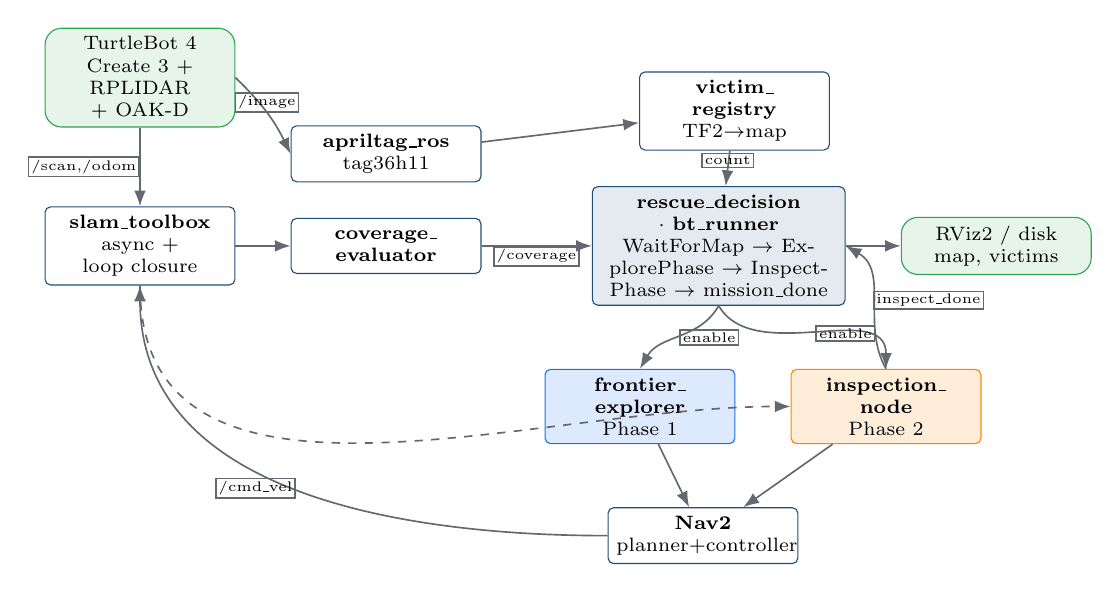
\begin{tikzpicture}[node distance=4.5mm and 7mm]
  \node[io] (robot) {TurtleBot~4\\\scriptsize Create~3 + RPLIDAR + OAK-D};
  \node[proc,below=10mm of robot] (slam) {\textbf{slam\_toolbox}\\\scriptsize async + loop closure};
  \node[proc,right=of slam] (metric) {\textbf{coverage\_}\\\textbf{evaluator}};
  \node[proc,above=of metric] (april) {\textbf{apriltag\_ros}\\\scriptsize tag36h11};
  \node[btnode,right=14mm of metric,text width=30mm] (bt) {\textbf{rescue\_decision $\cdot$ bt\_runner}\\\scriptsize WaitForMap $\to$ ExplorePhase $\to$ InspectPhase $\to$ mission\_done};
  \node[phase1,below=8mm of bt,xshift=-10mm] (explore) {\textbf{frontier\_}\\\textbf{explorer}\\\scriptsize Phase 1};
  \node[phase2,right=of explore] (inspect) {\textbf{inspection\_}\\\textbf{node}\\\scriptsize Phase 2};
  \node[proc,below=8mm of explore,xshift=8mm] (nav) {\textbf{Nav2}\\\scriptsize planner+controller};
  \node[proc,above=of bt,xshift=2mm] (reg) {\textbf{victim\_}\\\textbf{registry}\\\scriptsize TF2$\to$map};
  \node[io,right=of bt] (rviz) {RViz2 / disk\\\scriptsize map, victims};

  \draw[ar] (robot) -- node[arl,left]{/scan,/odom} (slam);
  \draw[ar] (robot.east) to[bend left=10] node[arl,above]{/image} (april.west);
  \draw[ar] (slam) -- (metric);
  \draw[ar] (april) -- (reg);
  \draw[ar] (metric) -- node[arl,below]{/coverage} (bt);
  \draw[ar] (bt.south) to[out=-120,in=60] node[arl,right]{enable} (explore.north);
  \draw[ar] (bt.south) to[out=-60,in=90] node[arl,right]{enable} (inspect.north);
  \draw[ar] (inspect.north) to[out=120,in=-30] node[arl,right]{inspect\_done} (bt.east);
  \draw[ar] (explore) -- (nav);
  \draw[ar] (inspect) -- (nav);
  \draw[ar] (nav.west) to[out=180,in=-90] node[arl,left]{/cmd\_vel} (slam.south);
  \draw[ar] (reg) -- node[arl,above]{count} (bt);
  \draw[ar] (bt) -- (rviz);
  \draw[ar,dashed] (slam) to[out=-90,in=180] (inspect.west);
\end{tikzpicture}
\caption{System architecture and topic flow. The Behavior Tree (\texttt{rescue\_decision}) is the
\emph{orchestrator}: it gates the Phase-1 explorer and the Phase-2 inspector via \texttt{/mission/*}
topics; the Python nodes do the work. SLAM feeds the map to exploration, coverage, Nav2 and inspection.}
\label{fig:arch}
\end{figure}

\noindent The packages and their responsibilities:
\begin{itemize}
\item \textbf{\texttt{rescue\_bringup}} - the \emph{one-click} entry point
(\texttt{bringup\_tb4.launch.py}) and all configs (Nav2, SLAM, AprilTag). A single launch starts
simulation, SLAM, Nav2, perception, the explorer/inspector and the Behavior Tree.
\item \textbf{\texttt{rescue\_robot}} - the Python ``megapackage'': \texttt{exploration/}
(frontier search + blacklist), \texttt{navigation/} (inspection planner + node), \texttt{detection/}
(victim registry/detector), \texttt{results/} (coverage evaluator + result exporter), and dev mocks.
\item \textbf{\texttt{rescue\_world}} - the Ignition Fortress arena (\texttt{rescue\_arena.sdf}) and
the voxel AprilTag targets. A \emph{single source} owns victim placement, so the map and the ground
truth never diverge.
\item \textbf{\texttt{rescue\_decision}} - the real C++ \texttt{BehaviorTree.CPP\,v3} runner
(visualisable in Groot), with the mission tree XML. This is the ``decision = BT, not FSM'' requirement.
\end{itemize}

\head{Perception pipeline.} Victims are \texttt{tag36h11} AprilTags (the assignment explicitly
excludes sophisticated human detection / YOLO). A subtle challenge: a PBR-textured tag renders
\emph{white} under Ogre2+Mesa, so \texttt{apriltag\_ros} sees nothing; we build each tag as
\textbf{voxel boxes} with a white quiet-zone ring around the native $8{\times}8$ marker (a naive
$10{\times}10$ resize destroys the quiet zone and makes the tag \emph{display but stay undetectable}).
Each detection yields a \texttt{camera}$\to$\texttt{victim}\_$i$ transform; \texttt{victim\_registry}
projects it to \texttt{map} via TF2, deduplicates by ID, and persists \texttt{results/victims.json} -
the ``report their coordinates in the global frame'' requirement.

% =================== 3. THEORETICAL FOUNDATIONS ===================
\section{Theoretical foundations (from the course)}\label{sec:concepts}
\head{SLAM and loop closure.} The robot builds the map online with \texttt{slam\_toolbox} (pose-graph
SLAM). Loop closure - emphasised in the course - corrects accumulated drift when the robot
re-observes a known place, keeping the global map consistent during repeated passes~[4,9].

\head{Frontier exploration and information gain (CM8).} A \emph{frontier} is the boundary between
free and unknown cells~[2]. Greedy selection takes the nearest frontier; \emph{information-gain}
selection maximises $\,g(f)=\mathrm{gain}(f)-\lambda\cdot\mathrm{cost}(f)\,$~[3], where $\mathrm{cost}$
is the \emph{Nav2 path length} (not Euclidean). Our $n{=}3$ benchmark confirms the theory: info-gain
reaches $0.85\pm0.08$ coverage (the only one above $90\,\%$) vs.\ $0.72$ for greedy. A key robustness
addition is an \emph{inaccessible-frontier blacklist} keyed by a quantized world coordinate, so a dead
frontier never gets reselected even as the grid origin shifts. Concretely, a frontier is blacklisted
either when Nav2 fails to reach it, or when it is re-selected \textbf{3 times in a row without any
coverage gain} (the common case in our arena); it is then never proposed again.

\begin{figure}[htbp]
\centering
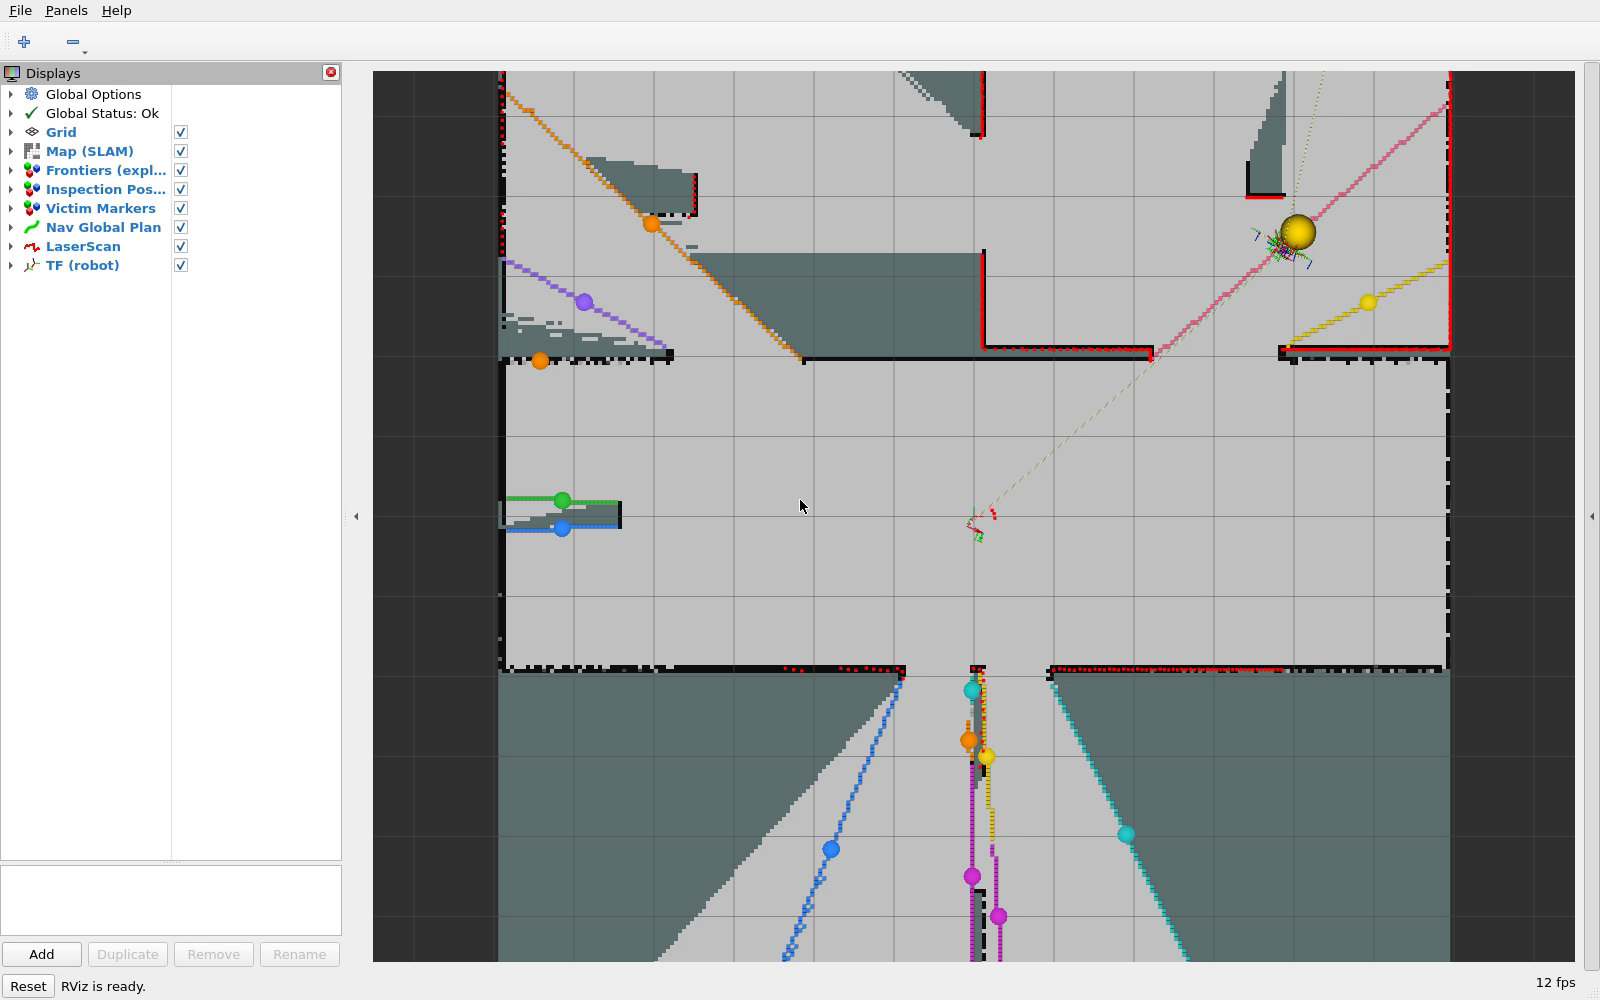
\includegraphics[width=0.72\linewidth]{rviz_frontiers}
\caption{Frontier exploration visualised in RViz (lab/TP style, CM8): the \emph{frontier cells} (the
free/unknown boundary) are coloured \textbf{per cluster} (connected-component segmentation), the yellow
sphere marks the best-utility goal frontier, and the blue line is the matching Nav2 plan. You \emph{see}
the coloured rim eat into the unknown up to $>90\,\%$ coverage (capture: \texttt{rviz\_capture.mp4}).}
\label{fig:rviz-frontiers}
\end{figure}

\head{Path planning and control (CM9--CM10).} The global planner produces a geometric path; the local
controller follows it. We compared \emph{Dijkstra/NavFn} vs.\ \emph{A* (Smac)}~[9]: in a tightly
partitioned arena the robot often stands inside the inflation layer, where A* refuses to plan
(``start in lethal space''); NavFn tolerates this and is kept. The controller is DWB (sampling-based,
CM10).

\begin{figure}[htbp]
\centering
\begin{subfigure}{0.40\linewidth}\centering
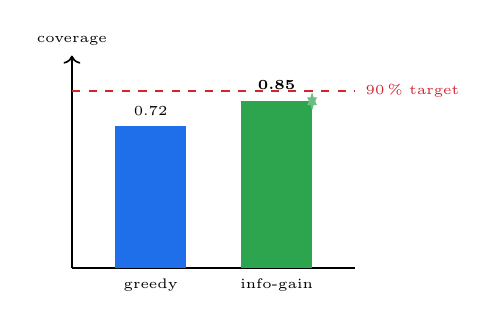
\begin{tikzpicture}[font=\scriptsize]
  \draw[->,semithick] (0,0)--(0,2.7) node[above,font=\tiny]{coverage};
  \draw[semithick] (0,0)--(3.6,0);
  \draw[dashed,nccred,thick] (0,2.25)--(3.6,2.25) node[right,font=\tiny,nccred]{90\,\% target};
  \fill[nccsky] (0.55,0) rectangle (1.45,1.80);
  \fill[nccgreen] (2.15,0) rectangle (3.05,2.12);
  \node[font=\tiny] at (1.0,-0.22){greedy}; \node[font=\tiny] at (1.0,2.0){0.72};
  \node[font=\tiny] at (2.6,-0.22){info-gain}; \node[font=\tiny] at (2.6,2.32){\textbf{0.85}};
  \draw[{Latex}-{Latex},nccgreen!70] (3.05,2.0)--(3.05,2.24);
\end{tikzpicture}
\caption{Bonus benchmark ($n{=}3$): information-gain is the only strategy above 90\,\% coverage.}
\end{subfigure}\hfill
\begin{subfigure}{0.56\linewidth}\centering\footnotesize
\begin{tabular}{@{}lll@{}}
\toprule
Planner & Property (CM9) & Status in \texttt{bl}\\
\midrule
Dijkstra/NavFn & optimal, explores all, tolerant & \textbf{chosen} (robust)\\
A* (Smac) & heuristic, faster, strict & tested, rejected here\\
RRT & fast, non-optimal & outlook\\
\bottomrule
\end{tabular}
\par\smallskip
\emph{Why NavFn:} in a partitioned arena the start is often in the inflation layer; A* aborts there,
NavFn does not.
\end{subfigure}
\caption{Exploration strategy (bonus) and global-planner comparison, grounded in the course.}
\label{fig:bench}
\end{figure}

\head{Coordinate frames and TF2.} A victim is detected in the \emph{camera} frame; \texttt{tf2}
chains $\text{camera}\to\text{victim}\_i\to\text{map}$ to report a global position (Fig.~\ref{fig:concepts}b),
exactly the ``project positions into the global frame'' requirement~[1,8].

\head{Behavior Trees vs.\ FSM.} The assignment forbids FSMs. A BT is reactive and composable: a memory
\texttt{Sequence} ticks children left-to-right, \emph{resumes} at the RUNNING node, and only advances
on SUCCESS - a real phase sequence rather than hand-rolled state transitions~[6].

\begin{figure}[htbp]
\centering
\begin{subfigure}{0.47\linewidth}\centering
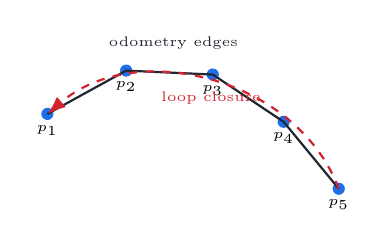
\begin{tikzpicture}[font=\scriptsize]
  \foreach \i/\x/\y in {1/0/0,2/1.0/0.55,3/2.1/0.5,4/3.0/-0.1,5/3.7/-0.95}{
     \fill[nccsky] (\x,\y) circle (2.2pt); \node[below=0.5pt,font=\tiny] at (\x,\y){$p_\i$};}
  \draw[nccdark,thick] (0,0)--(1.0,0.55)--(2.1,0.5)--(3.0,-0.1)--(3.7,-0.95);
  \node[font=\tiny,nccdark] at (1.6,0.9){odometry edges};
  \draw[dashed,nccred,-{Latex},thick] (3.7,-0.95) to[bend right=55] node[below,font=\tiny,nccred]{loop closure} (0,0);
\end{tikzpicture}
\caption{SLAM is a pose graph: re-observing a known place adds a \emph{loop-closure} edge that corrects
accumulated drift and keeps the global map consistent across repeated passes.}
\end{subfigure}\hfill
\begin{subfigure}{0.49\linewidth}\centering
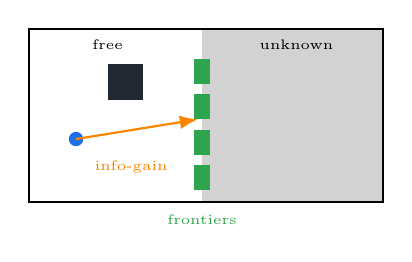
\begin{tikzpicture}[font=\scriptsize]
  \fill[gray!35] (2.2,0) rectangle (4.5,2.2);
  \draw[thick] (0,0) rectangle (4.5,2.2);
  \fill[nccdark] (1.0,1.3) rectangle (1.45,1.75);
  \foreach \y in {0.15,0.6,1.05,1.5} {\fill[nccgreen] (2.1,\y) rectangle (2.3,\y+0.32);}
  \fill[nccsky] (0.6,0.8) circle (2.6pt);
  \draw[-{Latex},nccorange,thick] (0.6,0.8)--(2.15,1.05);
  \node[font=\tiny] at (1.0,2.0){free}; \node[font=\tiny] at (3.4,2.0){unknown};
  \node[font=\tiny,nccgreen] at (2.2,-0.22){frontiers}; \node[font=\tiny,nccorange] at (1.3,0.45){info-gain};
\end{tikzpicture}
\caption{A \emph{frontier} is the free/unknown boundary (green); information-gain selects the most
informative one, scored by Nav2 \emph{path} cost (not Euclidean).}
\end{subfigure}
\caption{Two course concepts: pose-graph SLAM with loop closure (CM6--7) and frontier exploration
with information gain (CM8).}
\label{fig:course}
\end{figure}

\begin{figure}[htbp]
\centering
\begin{subfigure}{0.49\linewidth}\centering
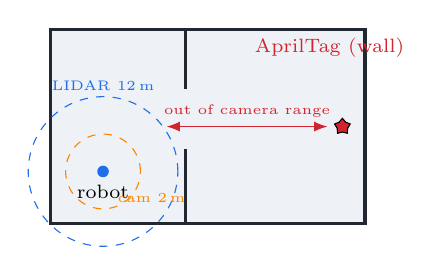
\begin{tikzpicture}[scale=0.95,every node/.style={font=\scriptsize}]
  % camera vs lidar gap
  \fill[nccgray] (0,0) rectangle (4.2,2.6);
  \draw[very thick,nccdark] (0,0) rectangle (4.2,2.6);
  \draw[very thick,nccdark] (1.8,2.6)--(1.8,1.8); \draw[very thick,nccdark] (1.8,0)--(1.8,1.0);
  \node[star,star points=5,fill=nccred,draw=black,inner sep=1.4pt] (tag) at (3.9,1.3) {};
  \node[right] at (2.6,2.35) {\color{nccred}AprilTag (wall)};
  \fill[nccsky] (0.7,0.7) circle (2.2pt); \node[below] at (0.7,0.65) {robot};
  \draw[dashed,nccsky] (0.7,0.7) circle (1.0cm); \node[nccsky] at (0.7,1.85){\tiny LIDAR 12\,m};
  \draw[nccorange,dashed] (0.7,0.7) circle (0.5cm); \node[nccorange] at (1.35,0.35){\tiny cam 2\,m};
  \draw[{Latex}-{Latex},nccred] (1.55,1.3)--(3.7,1.3) node[midway,above]{\tiny out of camera range};
\end{tikzpicture}
\caption{Camera-vs-LIDAR gap: LIDAR maps a room from the doorway, but the camera never gets within
2\,m of the wall tag $\Rightarrow$ pure exploration misses victims.}
\end{subfigure}\hfill
\begin{subfigure}{0.49\linewidth}\centering
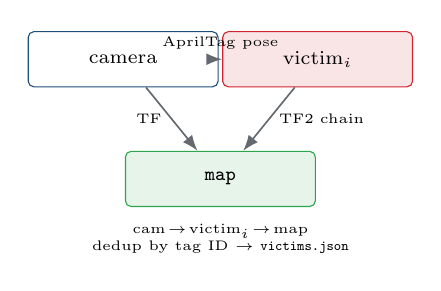
\begin{tikzpicture}[scale=0.95,every node/.style={font=\scriptsize}]
  \node[box,fill=white] (cam) at (0,0) {camera};
  \node[box,fill=nccred!12,draw=nccred] (vic) at (2.6,0) {victim$_i$};
  \node[box,fill=nccgreen!12,draw=nccgreen] (map) at (1.3,-1.6) {\texttt{map}};
  \draw[ar] (cam) -- node[above,font=\tiny]{AprilTag pose} (vic);
  \draw[ar] (cam) -- node[left,font=\tiny]{TF}(map);
  \draw[ar] (vic) -- node[right,font=\tiny]{TF2 chain}(map);
  \node[font=\tiny,align=center] at (1.3,-2.4){$\text{cam}\!\to\!\text{victim}_i\!\to\!\text{map}$\\dedup by tag ID $\to$ \texttt{victims.json}};
\end{tikzpicture}
\caption{TF2 projection of a detection into the global \texttt{map} frame.}
\end{subfigure}
\caption{Two core concepts behind the mission.}
\label{fig:concepts}
\end{figure}

\head{The two-phase mission.} Pure exploration completes the \emph{map} but caps victim detection
(Fig.~\ref{fig:concepts}a). The fix is a second \emph{autonomous} phase: from the map it just built,
\texttt{inspection\_node} derives \emph{one pose per discovered room} (facing the nearest wall, snapped
to a navigable cell, \emph{no victim coordinates}); the robot drives there and sweeps the camera. The
BT mission tree is the \texttt{Sequence}
\textsf{WaitForMap\,$\to$\,ExplorePhase\,$\to$\,InspectPhase\,$\to$\,VictimsFound\,$\to$\,mission\_done}
(Fig.~\ref{fig:bt}).

\begin{figure}[htbp]
\centering
\begin{subfigure}{0.34\linewidth}\centering
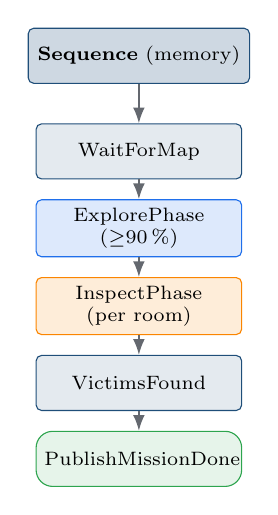
\begin{tikzpicture}[font=\scriptsize,node distance=3mm]
  \node[btnode,fill=nccblue!22,text width=26mm] (root) {\textbf{Sequence} (memory)};
  \node[btnode,below=5mm of root,text width=24mm] (n1) {WaitForMap};
  \node[phase1,below=2.5mm of n1,text width=24mm] (n2) {ExplorePhase ($\geq$90\,\%)};
  \node[phase2,below=2.5mm of n2,text width=24mm] (n3) {InspectPhase (per room)};
  \node[btnode,below=2.5mm of n3,text width=24mm] (n4) {VictimsFound};
  \node[io,below=2.5mm of n4,text width=24mm] (n5) {PublishMissionDone};
  \draw[ar] (root) -- (n1);
  \draw[ar] (n1) -- (n2); \draw[ar] (n2) -- (n3); \draw[ar] (n3) -- (n4); \draw[ar] (n4) -- (n5);
\end{tikzpicture}
\caption{Mission tree: a memory \texttt{Sequence} that resumes the RUNNING phase.}
\end{subfigure}\hfill
\begin{subfigure}{0.64\linewidth}\centering

\includegraphics[width=\linewidth]{algorithms_two_phase}
\caption{Algorithms in action. \emph{Left:} Phase~1 frontier exploration (blue path, green
info-gain goals). \emph{Right:} Phase~2 inspection (orange path, map-derived poses) catching the four
victims. Walls are drawn over the path, so it visibly threads the doorways.}
\end{subfigure}
\caption{The two-phase mission orchestrated by the Behavior Tree.}
\label{fig:bt}
\end{figure}

\head{Course concepts \emph{applied} in the project.} Table~\ref{tab:concepts} maps each lecture topic
to where it lives in our system - the project is essentially the course made concrete.

\begin{table}[htbp]\centering\footnotesize
\begin{tabular}{@{}p{0.30\linewidth}p{0.66\linewidth}@{}}
\toprule
\textbf{Course concept} & \textbf{Where it is applied in \texttt{bl}}\\
\midrule
SLAM + loop closure (CM6--7) & \texttt{slam\_toolbox} (async): online \texttt{/map} + \texttt{map}$\to$\texttt{odom} TF, loop closure on revisits\\
Frontier exploration (CM8) & \texttt{frontier\_explorer\_node}: free/unknown boundary, world-keyed blacklist\\
Information gain (CM8, bonus) & info-gain frontier selection; quantitative benchmark vs.\ greedy ($n{=}3$)\\
Path planning (CM9) & Nav2 global planner - NavFn (Dijkstra) kept; A* (Smac) compared\\
Local control (CM10) & Nav2 DWB controller (sampling-based trajectory scoring)\\
Coordinate frames / TF2 & \texttt{victim\_registry}: camera$\to$\texttt{victim}$_i\to$\texttt{map} projection\\
Behavior Trees (decision) & \texttt{rescue\_decision} (BT.CPP~v3): the two-phase mission orchestration\\
\bottomrule
\end{tabular}
\caption{The course concepts, and exactly where each one is applied in the project.}
\label{tab:concepts}
\end{table}

% =================== 4. DECISION JOURNEY ===================
\section{Decision journey: three representative runs}
The headline numbers - 97\,\% coverage, four victims, one click - hide a long and instructive road.
None of it came in one shot: almost every capability we now take for granted was, at some point, a run
that did the wrong thing for a reason we did not yet understand. We kept a written decision log in the
\emph{Problem $\to$ Investigation $\to$ Decision $\to$ Why} format, and the single most useful habit it
taught us was to \emph{measure before prescribing} - to let an event log or a metric, rather than an
intuition, tell us what was actually wrong. Three runs distill that story; each is reported below as
what \emph{blocked} and what we \emph{improved}, and Fig.~\ref{fig:journey} is the one-page overview.

\head{Run 1 - pure autonomous exploration (v20--v22).} Our first complete system did the obvious thing:
frontier exploration driving Nav2, with \texttt{slam\_toolbox} building the map underneath. It worked, in
the sense that it autonomously mapped some ninety percent of the building - but it kept finding only
about two of the four victims, and for a long time we could not see why. The answer turned out to be
geometric rather than algorithmic: a twelve-metre LIDAR maps a room comfortably from its doorway, so a
robot optimising for \emph{coverage} has no reason to walk up to a wall, yet the camera only recognises a
tag from about two metres. Exploration was therefore \emph{complete} and detection \emph{structurally
incomplete} at the same time. Along the way this run also taught us two sharp lessons - a frontier the
planner can never reach will trap the robot in an infinite loop unless it is blacklisted, and a
real-time factor low enough to starve the GPU camera renderer will silently stop detection while the
camera's metadata keeps flowing and hides the fault. We left this run with a clean map and dependable
autonomy, and a clear diagnosis of what was still missing.

\head{Run 2 - two-phase, BT-orchestrated (v32).} The fix followed directly from that diagnosis: if the
robot will not approach the walls while exploring, give it a second reason to. We added an
\emph{inspection} phase that reads the freshly built map, derives one pose per discovered room about
1.3\,m from the nearest wall - inside camera range, but using only the map and never the victims'
positions - and visits each in turn while sweeping the camera. Crucially, we also promoted the Behavior
Tree from a passive supervisor that merely watched the coverage metric into the genuine \emph{orchestrator}
of the mission, gating exploration and inspection in sequence; this is what makes the system conformant
to the ``decision by Behavior Tree, not FSM'' requirement in substance and not just in name. The result
was the breakthrough we had been chasing: \textbf{four victims out of four and 97\,\% coverage} in one
continuous, fully autonomous run.

\head{Run 3 - the final deliverable.} With the mission working, the last run was about turning a result
into a deliverable that is trustworthy and reproducible. We first asked whether we could simply run the
simulation faster: pushing the real-time factor to 1.5 did finish sooner, but it gave the camera less
time to settle at each pose and quietly dropped us back to three victims out of four, besides stressing
the GPU - so we kept the slower, reliable factor, a small reminder that for a deliverable, repeatability
outweighs speed. We then closed a set of presentation-grade issues that, while not affecting the robot's
behaviour, affected whether a reader could \emph{trust} the figures: the logged map-frame trajectory is
now drawn with the walls painted \emph{over} it, so the path is only ever visible in free space and
visibly threads each doorway (we verified that not one of its 568 segments crosses a wall); the
occupancy map is rendered with the correct vertical orientation, which had been the real reason an
earlier figure \emph{looked} as though the robot drove through walls; and each run's result files are
truncated on start, so the curves of one run no longer pile up on top of another's. The robustness work
that lets the inspection recover an unreachable pose on a teammate's machine (\S\ref{sec:concepts}) also
landed here. The outcome is the run this entire report draws on: \textbf{four victims out of four, about
97\,\% coverage}, a clean annotated map, a logged trajectory, and an HD capture of the live RViz
algorithms - a single, reproducible source for every figure shown.

\begin{figure*}[t]
\centering
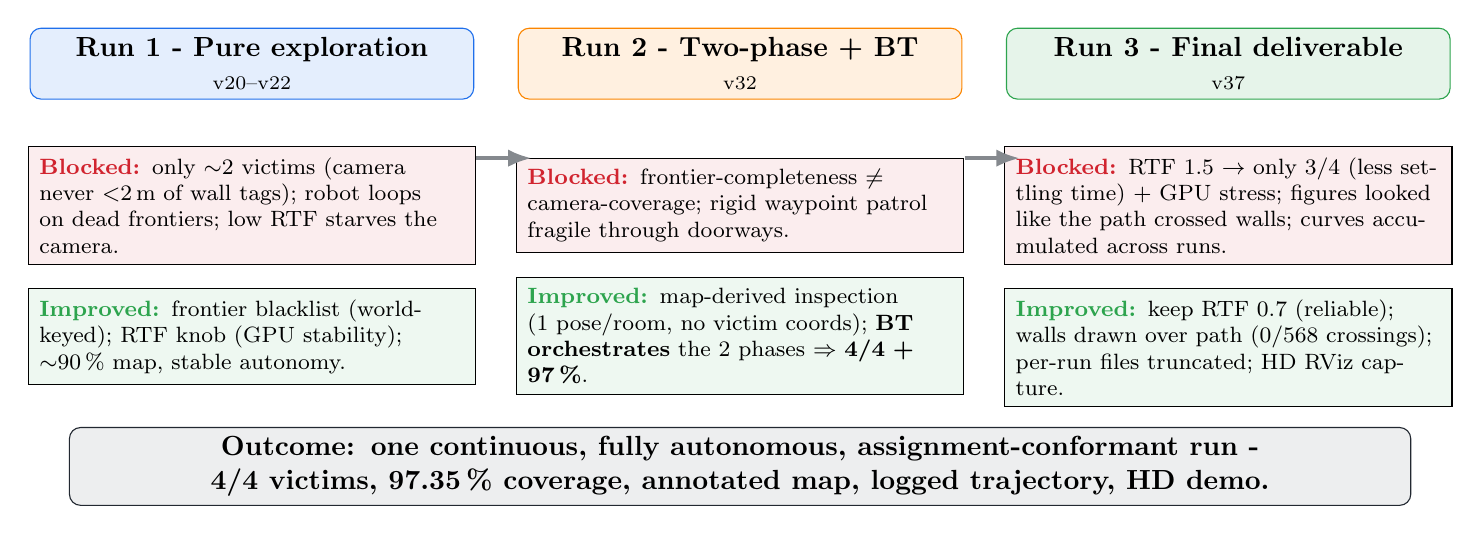
\begin{tikzpicture}[font=\footnotesize,node distance=3mm]
\definecolor{c1}{HTML}{1F6FEB}\definecolor{c2}{HTML}{FB8500}\definecolor{c3}{HTML}{2DA44E}
% three columns
\foreach \i/\x/\c/\title/\ver in {1/0/c1/{Run 1 - Pure exploration}/{v20–v22}, 2/6.2/c2/{Run 2 - Two-phase + BT}/{v32}, 3/12.4/c3/{Run 3 - Final deliverable}/{v37}} {
  \node[draw=\c,fill=\c!12,rounded corners,text width=5.4cm,minimum height=8mm,align=center,font=\bfseries] (h\i) at (\x+2.7,5.2) {\title\\\normalfont\scriptsize \ver};
}
% Run1 body
\node[draw,fill=nccred!8,text width=5.4cm,align=left,inner sep=4pt] (b0) at (2.7,3.4)
 {\textbf{\color{nccred}Blocked:} only $\sim$2 victims (camera never $<$2\,m of wall tags); robot loops on dead frontiers; low RTF starves the camera.};
\node[draw,fill=nccgreen!8,text width=5.4cm,align=left,below=of b0,inner sep=4pt] (i0)
 {\textbf{\color{nccgreen}Improved:} frontier blacklist (world-keyed); RTF knob (GPU stability); $\sim$90\,\% map, stable autonomy.};
% Run2 body
\node[draw,fill=nccred!8,text width=5.4cm,align=left,inner sep=4pt] (b1) at (8.9,3.4)
 {\textbf{\color{nccred}Blocked:} frontier-completeness $\neq$ camera-coverage; rigid waypoint patrol fragile through doorways.};
\node[draw,fill=nccgreen!8,text width=5.4cm,align=left,below=of b1,inner sep=4pt] (i1)
 {\textbf{\color{nccgreen}Improved:} map-derived inspection (1 pose/room, no victim coords); \textbf{BT orchestrates} the 2 phases $\Rightarrow$ \textbf{4/4 + 97\,\%}.};
% Run3 body
\node[draw,fill=nccred!8,text width=5.4cm,align=left,inner sep=4pt] (b2) at (15.1,3.4)
 {\textbf{\color{nccred}Blocked:} RTF~1.5 $\to$ only 3/4 (less settling time) + GPU stress; figures looked like the path crossed walls; curves accumulated across runs.};
\node[draw,fill=nccgreen!8,text width=5.4cm,align=left,below=of b2,inner sep=4pt] (i2)
 {\textbf{\color{nccgreen}Improved:} keep RTF~0.7 (reliable); walls drawn over path (0/568 crossings); per-run files truncated; HD RViz capture.};
\node[draw=nccdark,fill=nccdark!8,rounded corners,text width=16.8cm,align=center,below=4mm of i1,font=\bfseries] (res)
 {Outcome: one continuous, fully autonomous, assignment-conformant run - 4/4 victims, 97.35\,\% coverage, annotated map, logged trajectory, HD demo.};
\draw[-{Latex},very thick,nccdark!55] (5.55,4.0) -- (6.25,4.0);
\draw[-{Latex},very thick,nccdark!55] (11.75,4.0) -- (12.45,4.0);
\end{tikzpicture}
\caption{The decision journey on one page: three runs, each as \emph{what blocked} (red) $\to$
\emph{what we improved} (green). Two distinct root causes were unmasked late - the Nav2 cost
function discouraged entering rooms (fixed coverage), and a collapsed RTF starved the camera renderer
(fixed detection); the two-phase Behavior Tree then made 4/4 reliable.}
\label{fig:journey}
\end{figure*}

\subsection*{Challenges and solutions in detail}
Reaching 4/4 inside Run~1--2 meant peeling six \emph{stacked} causes - each fix revealed the next
(Table~\ref{tab:bugs}). The decisive insight: \emph{two} independent root causes hid under the
symptoms - the Nav2 cost function discouraged the robot from \emph{entering} rooms (a
\textbf{coverage} problem, fixed by lowering the inflation radius and cost scaling), and a collapsed
real-time factor \emph{starved the camera renderer} while \texttt{camera\_info} kept flowing (a
\textbf{detection} problem, very misleading). The two-phase Behavior Tree then made the result reliable.

\begin{table}[htbp]\centering\footnotesize
\begin{tabular}{@{}cp{0.31\linewidth}p{0.27\linewidth}p{0.30\linewidth}@{}}
\toprule
\# & Symptom & Root cause & Decision (fix)\\
\midrule
1 & Robot immobile, 0 victim & Patrol waypoints in \emph{unknown} space & Hybrid: explore first, \emph{then} act\\
2 & Waypoints rejected/blocking & Goals land on a wall & Validate goals in free space\\
3 & ``Failed to make progress'' & Create~3 safety reflex & \texttt{safety\_override=full}\\
4 & Deep corners rejected at 93\,\% & Corner cells still unknown & Goal-snapping to nearest free cell\\
5 & Inter-room routing fragile & No global path at goal time & Pivot: 360$^\circ$ spin-and-scan\\
6 & Only 1 victim detected & Low RTF starves camera renderer & Raise RTF; camera off while exploring\\
\bottomrule
\end{tabular}
\caption{Six stacked causes behind ``0 victims'', and the decision taken at each step.}
\label{tab:bugs}
\end{table}

\head{Host stability (WSL/GPU) - measure before prescribing.} Long runs rebooted the Windows host.
``Obvious'' culprits were wrong \emph{twice}: memory was fine (\texttt{free}: 5/19\,GiB) and no Windows
Update was pending. The event log revealed the real causes: GPU \texttt{VIDEO\_TDR\_FAILURE} /
\texttt{CLOCK\_WATCHDOG} bugchecks under sustained load. Our controllable fix is the
\textbf{real-time-factor knob} (\texttt{IA712\_GZ\_RT\_RATE}): staying on the GPU (software GL is
$\sim$23$\times$ slower) but lowering the physics/render cadence reduces sustained load without changing
\emph{simulated} time - so coverage and \texttt{time\_to\_90} are unaffected.

% =================== 5. TEAM / GIT ===================
\section{Team collaboration and task distribution}
We worked on per-member \texttt{dev/*} branches integrated into \texttt{dev/bl}
(Fig.~\ref{fig:branches}); \texttt{bl} is the merged version this report describes.

\begin{figure}[htbp]
\centering
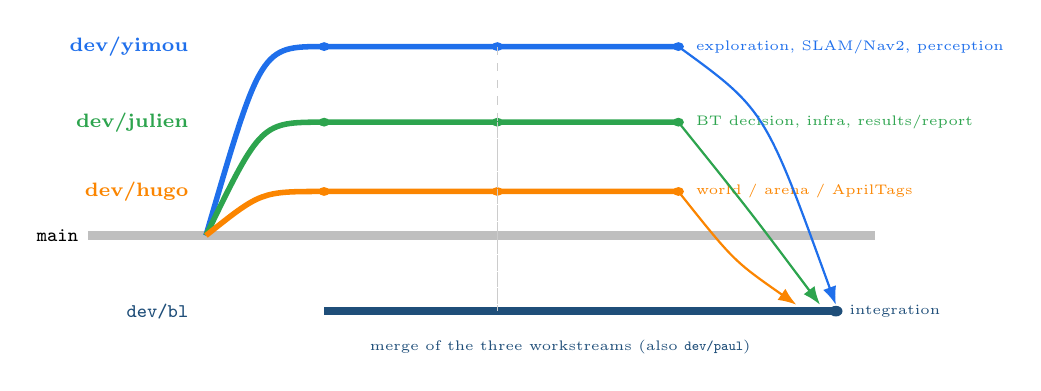
\begin{tikzpicture}[font=\scriptsize,xscale=1.0,yscale=0.8]
  \draw[gray!50,line width=3pt] (0,0) -- (10,0); \node[left] at (0,0){\texttt{main}};
  % feature branches
  \foreach \y/\name/\c in {3.0/{dev/yimou}/nccsky, 1.8/{dev/julien}/nccgreen, 0.7/{dev/hugo}/nccorange} {
     \draw[\c,line width=2pt] (1.5,0) .. controls (2.2,\y) .. (3.0,\y) -- (7.5,\y);
     \node[\c,left,font=\scriptsize\bfseries] at (1.4,\y) {\name};
     \fill[\c] (3.0,\y) circle (2pt); \fill[\c] (5.2,\y) circle (2pt); \fill[\c] (7.5,\y) circle (2pt);
  }
  \node[nccsky,right,font=\tiny] at (7.6,3.0){exploration, SLAM/Nav2, perception};
  \node[nccgreen,right,font=\tiny] at (7.6,1.8){BT decision, infra, results/report};
  \node[nccorange,right,font=\tiny] at (7.6,0.7){world / arena / AprilTags};
  % bl integration branch
  \draw[nccblue,line width=3pt] (3.0,-1.2) -- (9.5,-1.2);
  \node[nccblue,left,font=\scriptsize\bfseries] at (1.4,-1.2){\texttt{dev/bl}};
  \node[nccblue,right,font=\tiny] at (9.55,-1.2){integration};
  \foreach \y in {3.0,1.8,0.7} { \draw[dashed,gray!40] (5.2,\y) -- (5.2,-1.2); }
  \draw[-{Latex},nccsky,thick] (7.5,3.0) .. controls (8.6,2) .. (9.5,-1.1);
  \draw[-{Latex},nccgreen,thick] (7.5,1.8) .. controls (8.4,0.4) .. (9.3,-1.1);
  \draw[-{Latex},nccorange,thick] (7.5,0.7) .. controls (8.2,-0.4) .. (9.0,-1.1);
  \fill[nccblue] (9.5,-1.2) circle (2.4pt);
  \node[below,font=\tiny,nccblue] at (6,-1.5){merge of the three workstreams (also \texttt{dev/paul})};
\end{tikzpicture}
\caption{Branch construction: three per-developer feature branches (workstreams from the git history)
are merged into \texttt{dev/bl}, the integration branch.}
\label{fig:branches}
\end{figure}

\noindent{\footnotesize\textbf{Task distribution} (from the git history):
\textbf{Yimou ZHANG} - autonomous exploration, SLAM/Nav2 wiring, perception core, benchmark;
\textbf{Julien GIMENEZ} - Behavior-Tree decision \& two-phase orchestration, simulation infrastructure
(WSL/GPU/RTF/DDS), results, integration (\texttt{bl}) and report;
\textbf{Hugo FANCHINI} - simulation world, rescue arena and AprilTag target placement
(\texttt{rescue\_world});
\textbf{Paul CINTRA} - perception/detection support and testing (\texttt{dev/paul}).}

% =================== 6. RESULTS ===================
\section{Results}
Fig.~\ref{fig:seq} shows the live RViz algorithms across the mission; Fig.~\ref{fig:results} the
deliverable artefacts. All come from the single final run (\texttt{results/examples/l18\_nominal}).

\begin{figure}[htbp]
\centering
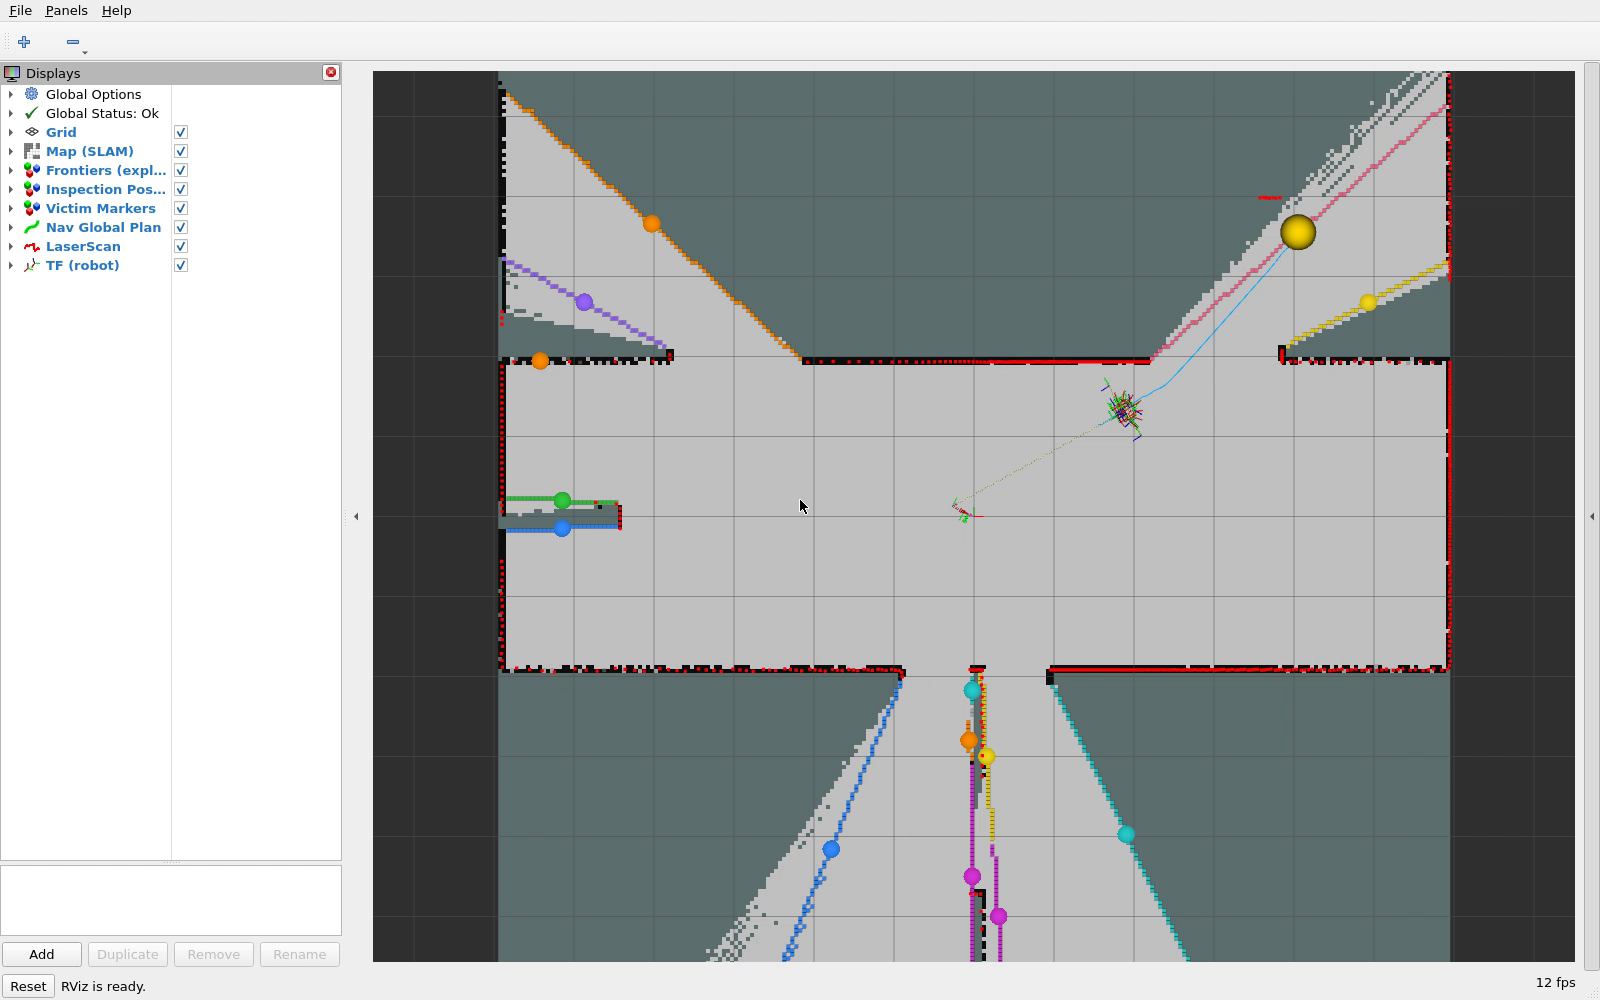
\includegraphics[width=0.315\linewidth]{rviz_seq_1}\hfill
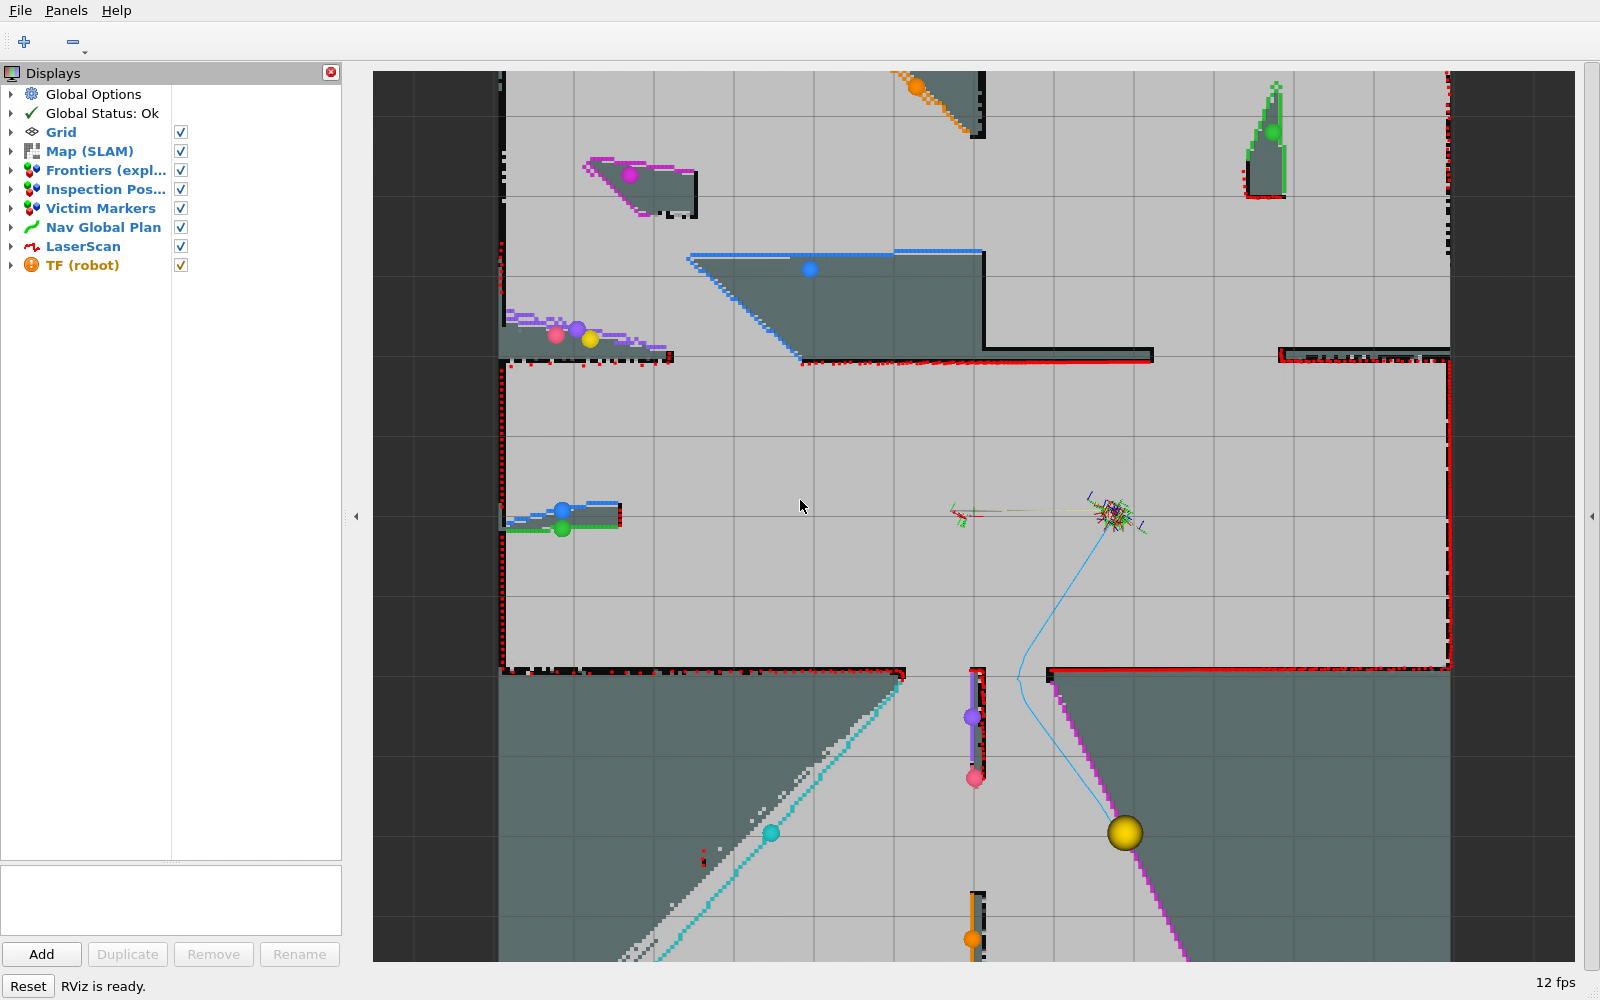
\includegraphics[width=0.315\linewidth]{rviz_seq_2}\hfill

\includegraphics[width=0.315\linewidth]{rviz_seq_3}\\[3pt]
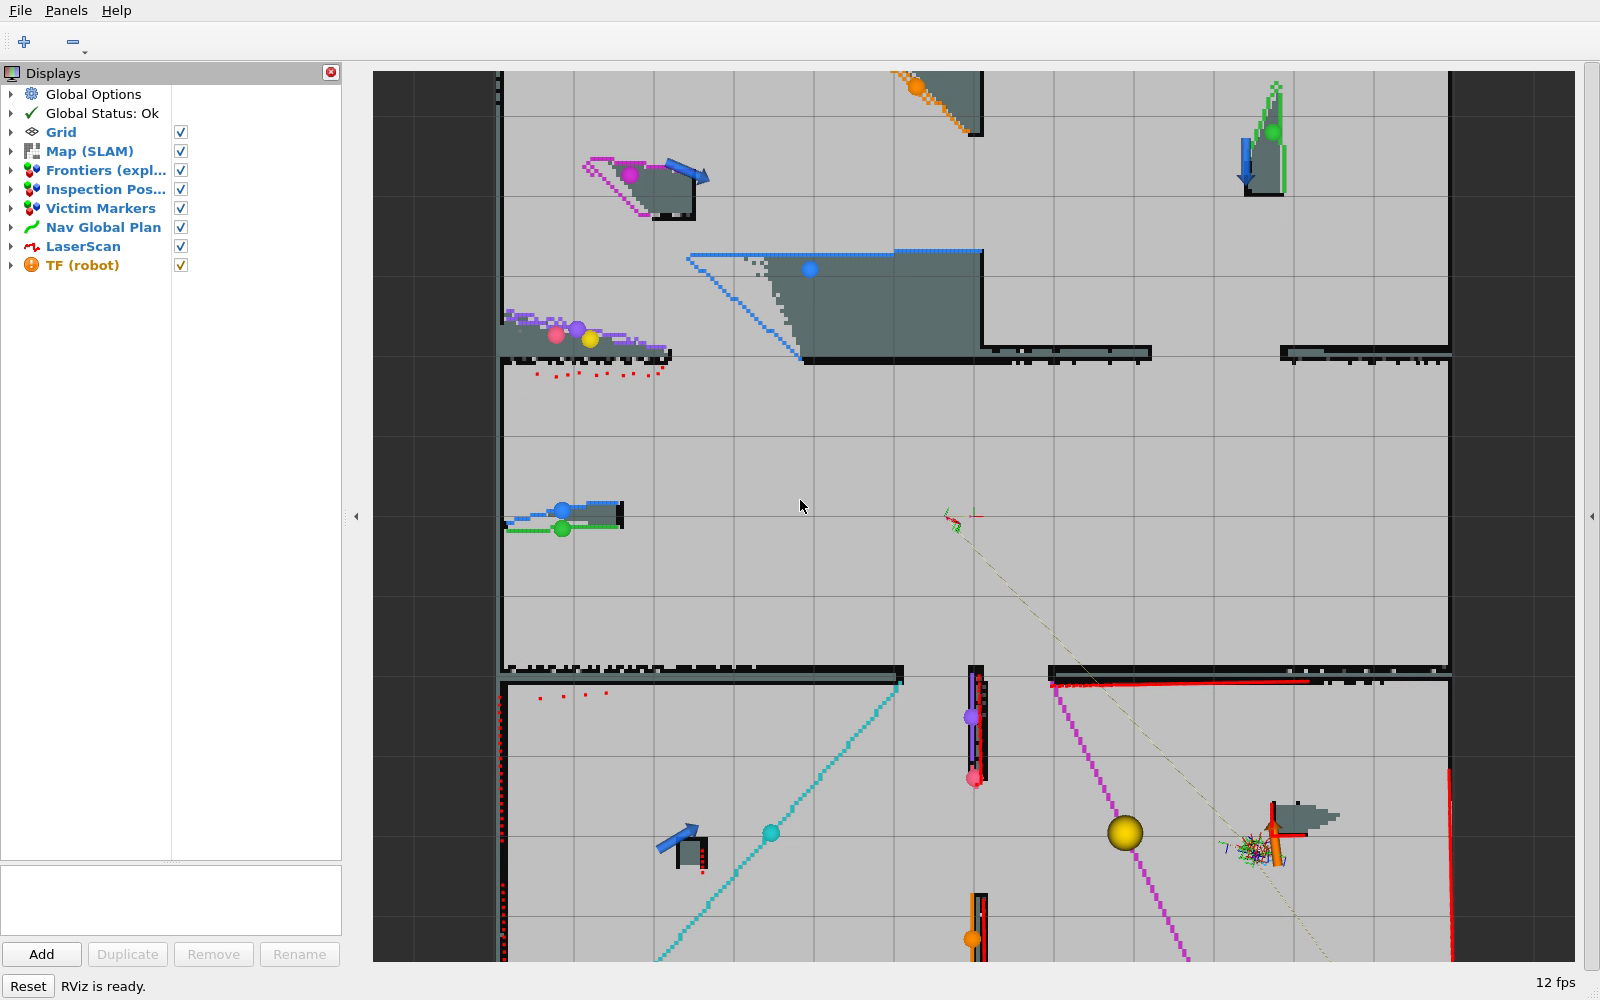
\includegraphics[width=0.315\linewidth]{rviz_seq_4}\hfill

\includegraphics[width=0.315\linewidth]{rviz_seq_5}\hfill
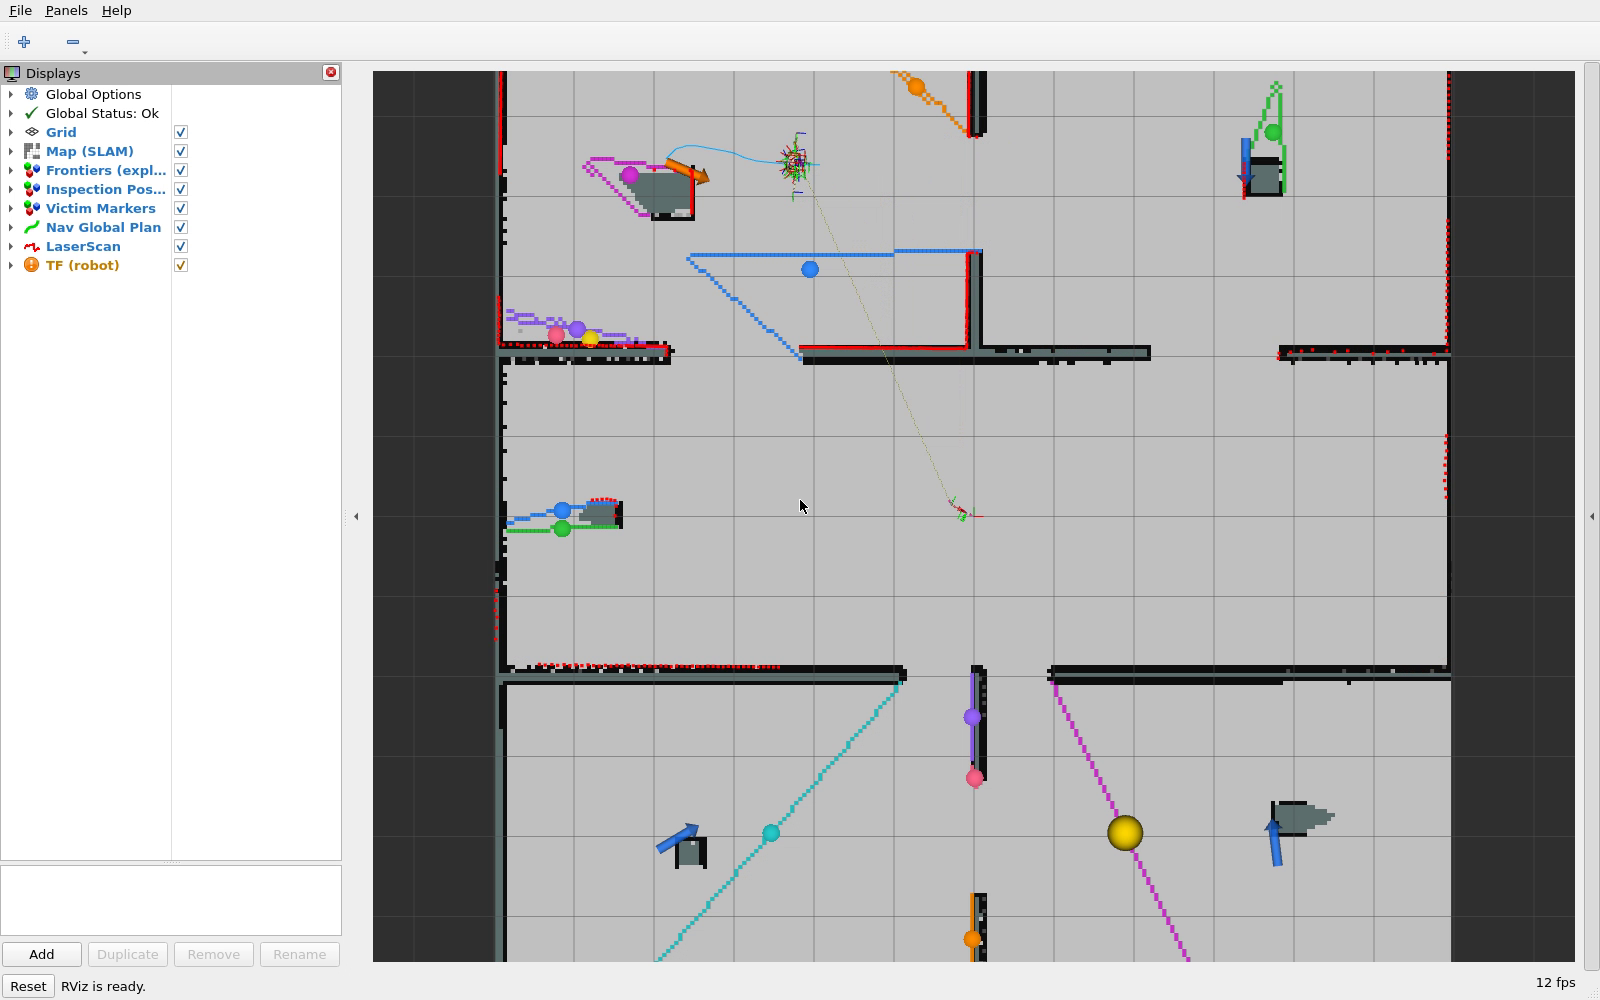
\includegraphics[width=0.315\linewidth]{rviz_seq_6}
\caption{Live RViz at six key moments (1--3: early exploration, map nearly built, phase transition;
4--6: room inspection, victims appearing, final map) - showing the map (SLAM), frontiers, inspection
poses, Nav2 plan, LaserScan and the four victim markers. Captured at HD on a virtual X server.}
\label{fig:seq}
\end{figure}

\begin{figure}[htbp]
\centering
\begin{subfigure}{0.33\linewidth}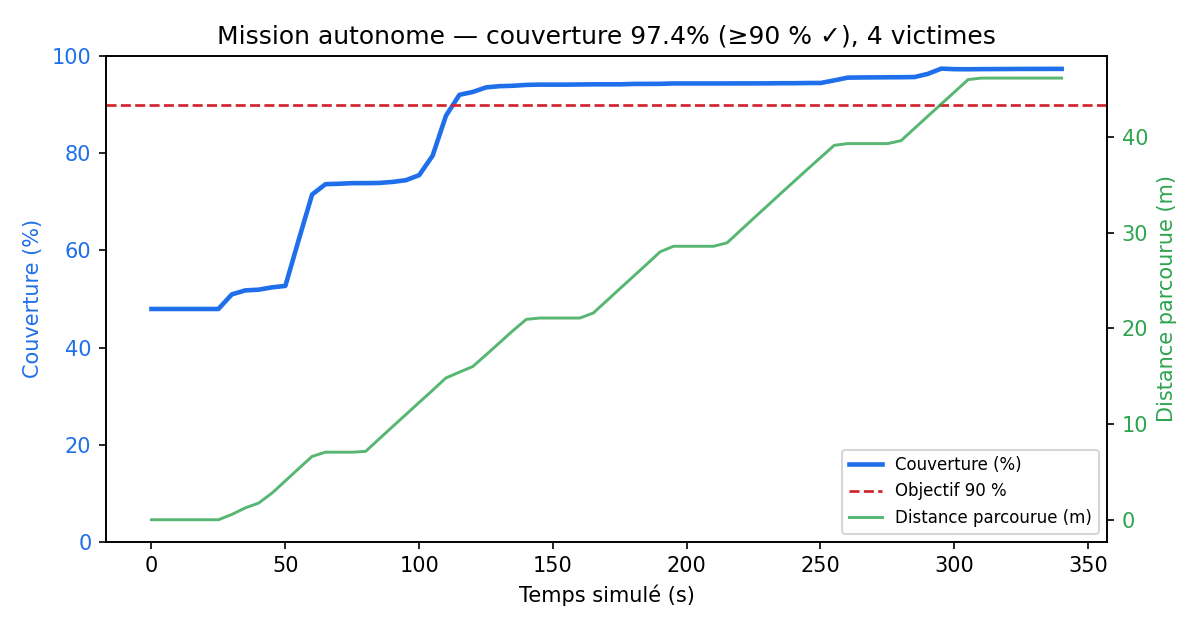
\includegraphics[width=\linewidth]{coverage_curve}\caption{Coverage \& path vs.\ time (90\,\% target).}\end{subfigure}\hfill
\begin{subfigure}{0.33\linewidth}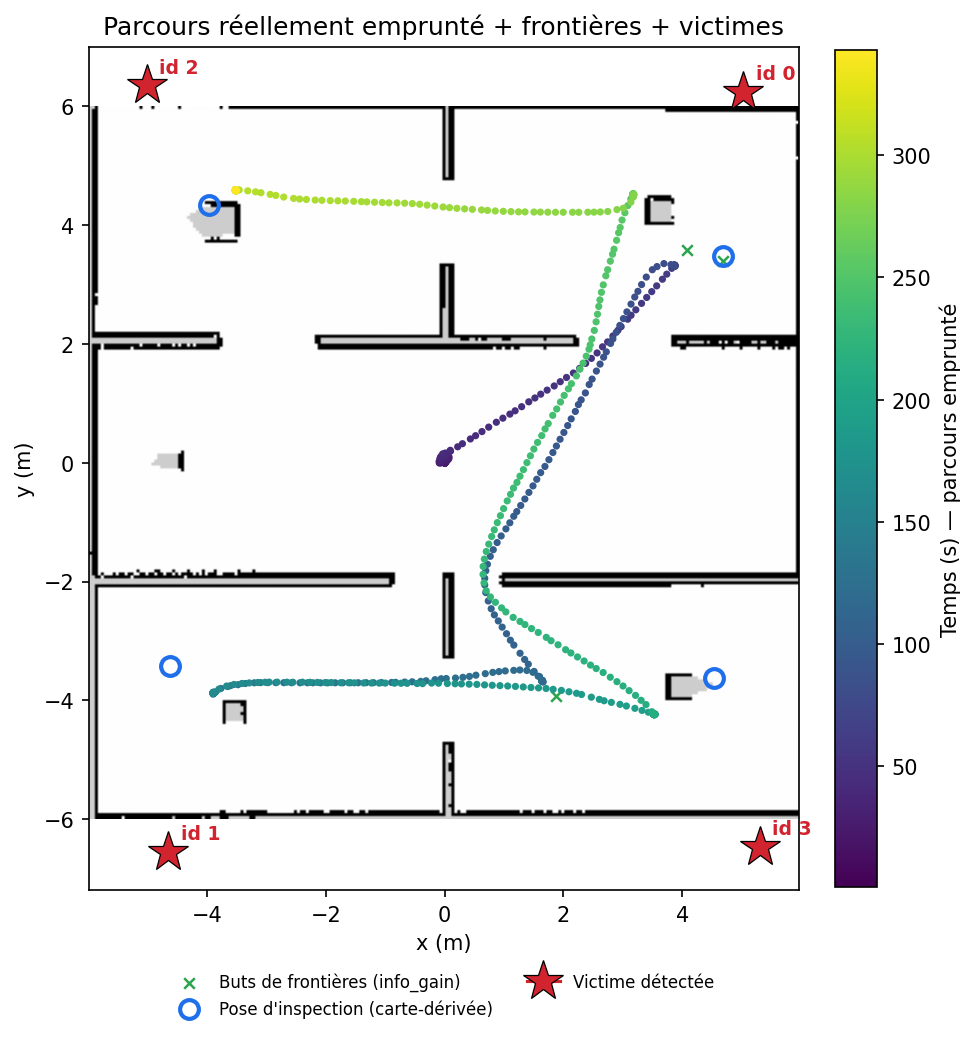
\includegraphics[width=\linewidth]{trajectory_map}\caption{Real path (time-coloured), threading doorways.}\end{subfigure}\hfill
\begin{subfigure}{0.32\linewidth}
\includegraphics[width=\linewidth]{mission_map}\caption{Final map: 4 victims + inspection tour.}\end{subfigure}
\caption{Quantitative results: \textbf{97.35\,\%} coverage and \textbf{4/4} victims, fully autonomous.
The trajectory is the actual map-frame path; walls are drawn over it, so it visibly passes through
doorways (verified: no segment crosses a wall).}
\label{fig:results}
\end{figure}

\begin{figure}[htbp]
\centering
\begin{subfigure}{0.49\linewidth}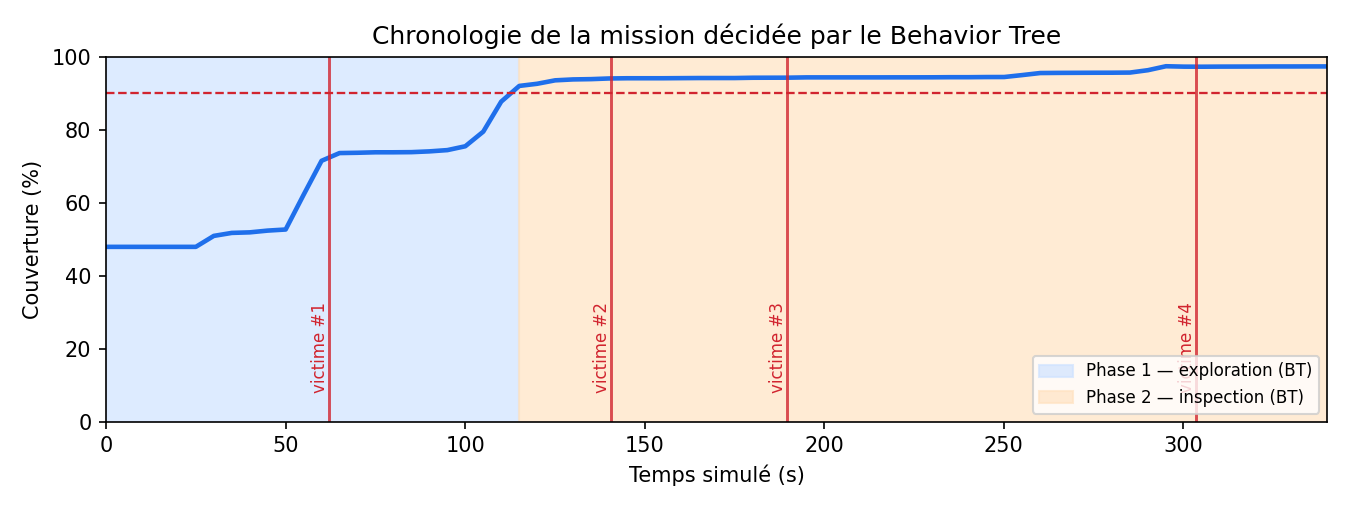
\includegraphics[width=\linewidth]{mission_timeline}\caption{BT-decided timeline: Phase~1 (blue) / Phase~2 (orange) bands and the instant each victim is detected.}\end{subfigure}\hfill
\begin{subfigure}{0.30\linewidth}
\includegraphics[width=\linewidth]{annotated_map_hd}\caption{Deliverable: final map marked with the victims.}\end{subfigure}\hfill
\begin{subfigure}{0.185\linewidth}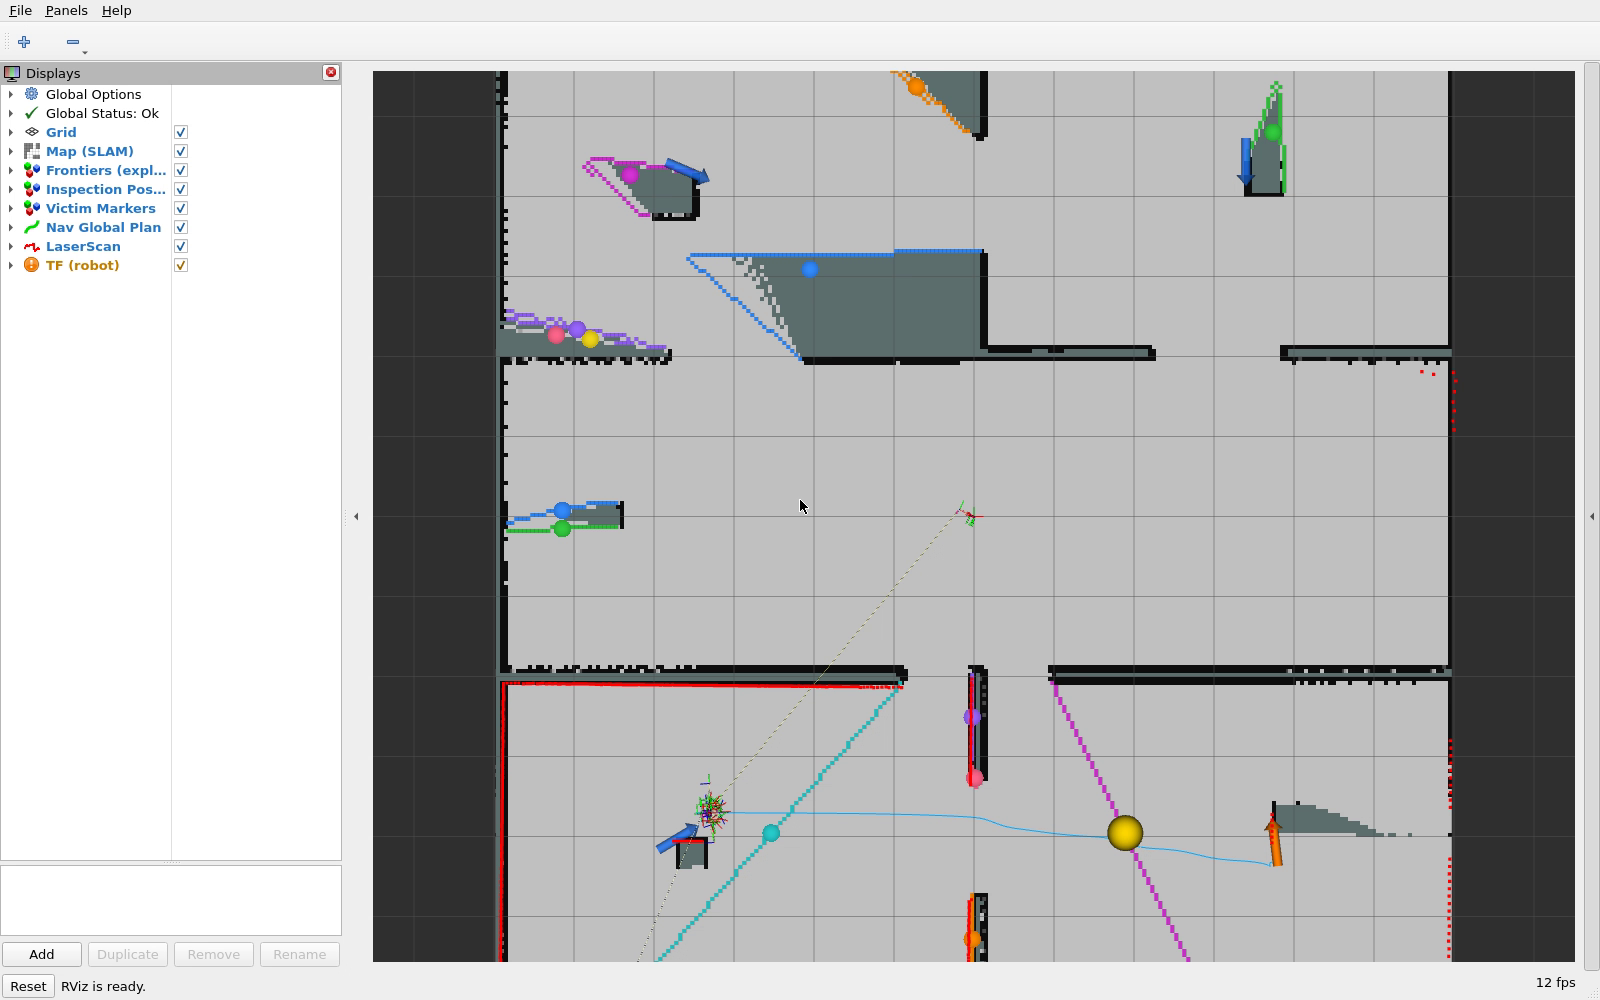
\includegraphics[width=\linewidth]{rviz_live}\caption{Live RViz.}\end{subfigure}
\caption{Mission chronology and the assignment deliverable (``final map marked with all victim
positions''). The phase split and victim-detection instants confirm the BT orchestration.}
\label{fig:timeline}
\end{figure}

\begin{figure}[htbp]
\centering

\includegraphics[width=0.92\linewidth]{mission_summary}
\caption{One-glance summary montage: final map with the four victims and the inspection tour
(top-left), the real time-coloured trajectory (top-right), coverage and path length over time
(bottom-left), and the deliverable annotated map (bottom-right). Everything is regenerated from the
single archived run, so the figures are reproducible from data.}
\label{fig:montage}
\end{figure}

\head{Reading the results.} The coverage curve (Fig.~\ref{fig:results}a) shows the two phases clearly:
a fast rise during exploration up to the 90\,\% target, then a plateau during inspection while the
path length keeps growing (the robot still moves, room to room, but the map is already complete). The
mission timeline (Fig.~\ref{fig:timeline}a) overlays the four victim-detection instants on the phase
bands: the first victims are caught \emph{during} exploration when the robot happens to pass close to a
wall tag, and the remaining ones \emph{during} inspection - exactly the behaviour the two-phase design
predicts. The trajectory (Fig.~\ref{fig:results}b) confirms the robot visits all four rooms and returns,
threading every doorway.

\head{Running and reproducibility.} The whole stack starts with one command,
\texttt{ros2 launch rescue\_bringup bringup\_tb4.launch.py}. The nominal run is archived
(\texttt{results/examples/l18\_nominal}) so every figure in this report is regenerable from data; the
bonus benchmark is \emph{resumable} (each run persists its summary, valid runs are skipped on restart),
which is how the campaign survived the host reboots. RViz is captured to HD video on a headless
machine via a virtual X server, giving the live-algorithm sequence of Fig.~\ref{fig:seq}.

% =================== 7. LESSONS + TIMELINE ===================
\section{Lessons learned and timeline}
\head{Lessons learned.} Four lessons stand out, and they are as much about engineering method as about
robotics. The first is to \emph{measure before prescribing}. Twice we were certain we knew why the host
machine kept rebooting - it had to be memory, then surely a pending Windows Update - and twice we
were wrong; only the event log, \texttt{free} and \texttt{nvidia-smi} pointed at the real culprits, a GPU
thermal-driver crash and, separately, a camera renderer starved by a collapsed real-time factor while
its metadata kept flowing and hid the problem. The second lesson is that \emph{one fix reveals the next}:
getting from zero to four victims meant peeling six stacked causes - an unmapped goal, a goal on a
wall, a safety reflex, an unreachable corner, fragile inter-room routing, and finally the starved camera
- where each correction simply exposed the one beneath it. The third is that \emph{robust beats rigid}:
in a partitioned arena, an adaptive explorer that already visits every room, followed by a full
360$^\circ$ camera sweep, consistently beats a hand-authored waypoint patrol that breaks the moment the
map differs slightly. And the fourth is \emph{conformity by design} - by making the Behavior Tree truly
\emph{orchestrate} the mission rather than merely watch it, we satisfy the assignment's ``decision by BT,
not FSM'' requirement in spirit and not only on paper.

\head{Timeline (L13--L18).} The project followed the suggested schedule (Fig.~\ref{fig:timelineL}).

\begin{figure}[htbp]
\centering
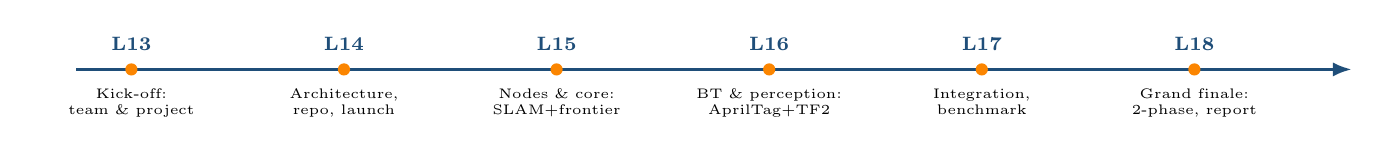
\begin{tikzpicture}[font=\scriptsize]
  \draw[line width=1.2pt,nccblue,-{Latex[length=2.4mm]}] (0,0) -- (16.2,0);
  \foreach \x/\l/\d in {0.3/L13/{Kick-off:\\team \& project}, 3/L14/{Architecture,\\repo, launch}, 5.7/L15/{Nodes \& core:\\SLAM+frontier}, 8.4/L16/{BT \& perception:\\AprilTag+TF2}, 11.1/L17/{Integration,\\benchmark}, 13.8/L18/{Grand finale:\\2-phase, report}} {
     \fill[nccorange] (\x+0.4,0) circle (2.2pt);
     \node[above,nccblue,font=\scriptsize\bfseries] at (\x+0.4,0.12){\l};
     \node[below,align=center,font=\tiny,text width=24mm] at (\x+0.4,-0.12){\d};
  }
\end{tikzpicture}
\caption{The six sessions L13--L18 and their milestones.}
\label{fig:timelineL}
\end{figure}

\section{Discussion and conclusion}
Looking back, the project succeeds less because of any single clever algorithm than because of how the
pieces are made to cooperate. The exploration is a textbook frontier search, the planner and controller
are stock Nav2 plugins, the SLAM is \texttt{slam\_toolbox} out of the box, and the detector is
\texttt{apriltag\_ros}; what we contributed is the \emph{integration} - a Behavior Tree that turns
these independent components into a coherent mission, and a second autonomous phase that closes the gap
between ``the map is complete'' and ``every victim is found''. This is exactly the shift the assignment
asks for: from writing code that merely runs to engineering a system whose parts hold together under
real conditions.

The two-phase design is the conceptual heart of the result. A robot that only explores will, in a
partitioned building, map each room comfortably from its doorway with a twelve-metre LIDAR and never
need to step inside - which is efficient for mapping but fatal for a camera that only sees a tag from
two metres. Separating \emph{mapping} from \emph{inspection}, and deriving the inspection poses from the
map the robot has just built rather than from any prior knowledge of the victims, keeps the system
fully autonomous while making detection reliable. The Behavior Tree is what makes this separation clean:
each phase is a node that runs until its own success condition, and the mission simply reads as a
sequence.

Robustness, finally, was a lesson in itself. A run that works on one machine is not the same as a system
that works: a slightly different costmap on a teammate's computer was enough to make two inspection poses
unreachable, until the inspector learned to wait for the costmap to settle and to fall back to a pose
pulled into the room's interior. The honest conclusion of this project is therefore as much about method
- measure, isolate one cause at a time, make the system tolerant rather than rigid - as it is about
the final numbers. Natural next steps would be to compare A* against NavFn on a less aggressive costmap,
to try a Regulated Pure Pursuit controller for smoother doorway traversals, and to add a second robot
and let the Behavior Tree coordinate a shared map.

\section*{Acknowledgements}
We warmly thank \textbf{Zhi Yan}, Teacher-Researcher at ENSTA, for the IA712 course and guidance that
made this project possible.

% =================== REFERENCES ===================
\begingroup
\small
\begin{thebibliography}{99}
\setlength{\itemsep}{0pt}
\bibitem{assign} IA712 Mobile Robotics - Final Project, Project~B (assignment). Course site: \url{https://yzrobot.github.io/IA712/}.
\bibitem{yamauchi} B.~Yamauchi, \emph{A frontier-based approach for autonomous exploration}, IEEE CIRA, 1997.
\bibitem{stachniss} C.~Stachniss et al., \emph{Information gain-based exploration using Rao-Blackwellized particle filters}, ICRA, 2005.
\bibitem{slamtb} S.~Macenski, I.~Jambrecic, \emph{slam\_toolbox: SLAM for the dynamic world}, JOSS, 2021.
\bibitem{nav2} S.~Macenski et al., \emph{The Marathon~2: A navigation system (Nav2)}, IROS, 2020.
\bibitem{btcpp} D.~Faconti et al., \emph{BehaviorTree.CPP} library, \url{https://www.behaviortree.dev/}.
\bibitem{apriltag} E.~Olson, \emph{AprilTag: A robust and flexible visual fiducial system}, ICRA, 2011; \texttt{apriltag\_ros}.
\bibitem{tf2} T.~Foote, \emph{tf2: The transform library}, IEEE TePRA, 2013.
\bibitem{cm} IA712 lecture notes (CM6--CM10: SLAM, Exploration, Path Planning, Control), \url{https://yzrobot.github.io/IA712/}.
\bibitem{repo} Project repository, \url{https://github.com/YiZeems/autonomous-search-and-rescue}.
\end{thebibliography}
\endgroup

\end{document}
